\documentclass{article}
\usepackage{amsmath,amssymb,amsfonts,amsthm,latexsym}
\usepackage{tikz,tikz-network}
\usetikzlibrary{calc, math}
\usetikzlibrary{decorations.markings}

\begin{document}

	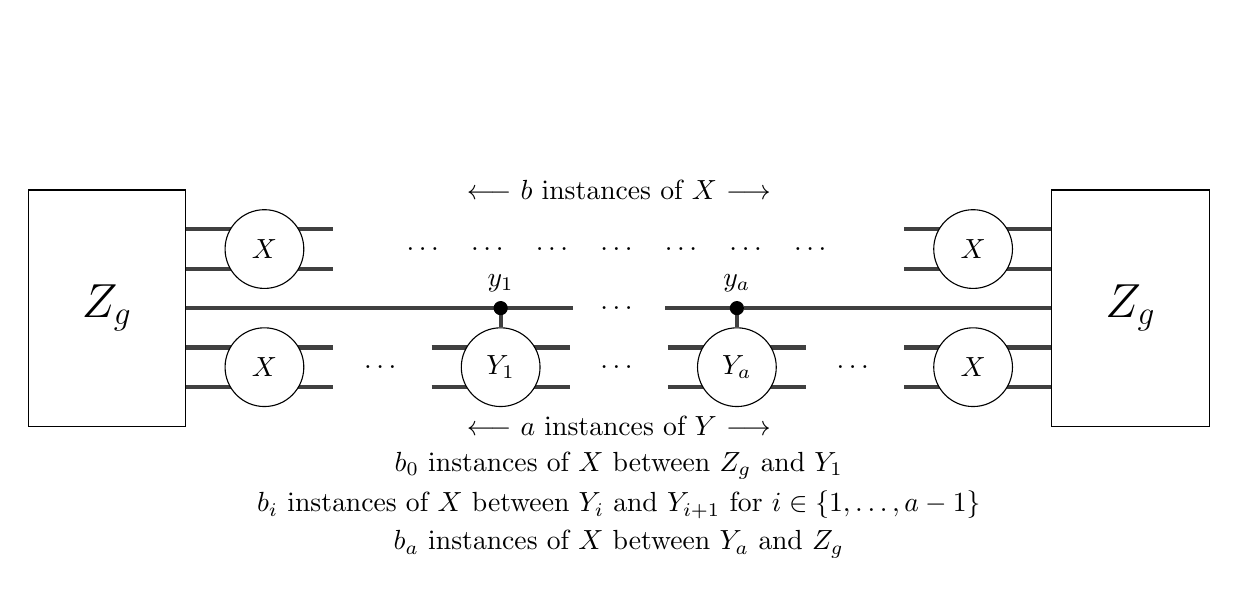
\begin{tikzpicture}[every node/.style={draw,shape=rectangle,fill=black,text=white},scale=1]
		\node[rectangle,draw,fill=white,text=black,minimum width = 2cm, minimum height = 3cm] (zg1) at (0,0) {\LARGE $Z_g$};	
		\node[rectangle,draw,fill=white,text=black,minimum width = 2cm, minimum height = 3cm] (zg2) at (13,0) {\LARGE $Z_g$};

		\node[fill=none,draw=none] (zg11) at (0,1) {};
		\node[fill=none,draw=none] (zg12) at (0,0.5) {};
		\node[fill=none,draw=none] (zg13) at (0,0) {};
		\node[fill=none,draw=none] (zg14) at (0,-0.5) {};
		\node[fill=none,draw=none] (zg15) at (0,-1) {};

		\node[fill=none,draw=none] (zg21) at (13,1) {};
		\node[fill=none,draw=none] (zg22) at (13,0.5) {};
		\node[fill=none,draw=none] (zg23) at (13,0) {};
		\node[fill=none,draw=none] (zg24) at (13,-0.5) {};
		\node[fill=none,draw=none] (zg25) at (13,-1) {};



		\node[circle,draw,fill=white,text=black,minimum width = 1cm, minimum height = 1cm] (x11) at (2,0.75) {$X$};
		\node[circle,draw,fill=white,text=black,minimum width = 1cm, minimum height = 1cm] (x12) at (2,-0.75) {$X$};

		\node[circle,draw,fill=white,text=black,minimum width = 1cm, minimum height = 1cm] (x21) at (11,0.75) {$X$};
		\node[circle,draw,fill=white,text=black,minimum width = 1cm, minimum height = 1cm] (x22) at (11,-0.75) {$X$};

		\node[circle,draw=none,fill=none,text=black] (text1) at (6.5,1.5) {$\longleftarrow$ $b$ instances of $X$ $\longrightarrow$};
		\node[circle,draw=none,fill=none,text=black] (text1) at (6.5,0.75) {$\dots$ \ \ $\dots$ \ \ $\dots$ \ \ $\dots$ \ \ $\dots$ \ \ $\dots$ \ \ $\dots$};



		\node[fill=black,draw,shape=circle,scale=0.5,label={[color=black]above:$y_1$}] (y1) at (5,0) {};
		\node[fill=black,draw,shape=circle,scale=0.5,label={[color=black]above:$y_a$}] (y2) at (8,0) {};

		\node[circle,draw,fill=white,text=black,minimum width = 1cm, minimum height = 1cm] (y11) at (5,-0.75) {$Y_1$};
		\node[circle,draw,fill=white,text=black,minimum width = 1cm, minimum height = 1cm] (y22) at (8,-0.75) {$Y_a$};

		\Edge[,bend=0](y1)(y11)
		\Edge[,bend=0](y2)(y22)	

		\Edge[,bend=0](zg13)(y1)
		\Edge[,bend=0](zg23)(y2)

		\node[fill=none,draw=none,shape=circle,scale=0.5] (w1) at (6,0) {};
		\node[fill=none,draw=none,shape=circle,scale=0.5] (w2) at (7,0) {};
		\node[fill=none,draw=none,text=black,shape=circle,scale=1] (w3) at (6.5,0) {$\dots$};
		\node[fill=none,draw=none,text=black,shape=circle,scale=1] (w4) at (6.5,-0.75) {$\dots$};

		\node[fill=none,draw=none,text=black,shape=circle,scale=1] (w5) at (3.5,-0.75) {$\dots$};
		\node[fill=none,draw=none,text=black,shape=circle,scale=1] (w6) at (9.5,-0.75) {$\dots$};

		\Edge[,bend=0](y1)(w1)
		\Edge[,bend=0](y2)(w2)

		\node[rectangle,draw=none,fill=none,text=black] (text2) at (6.5,-1.5) {$\longleftarrow$ $a$ instances of $Y$ $\longrightarrow$};
		\node[rectangle,draw=none,fill=none,text=black] (text2) at (6.5,-2) {$b_0$ instances of $X$ between $Z_g$ and $Y_1$}; 
		\node[rectangle,draw=none,fill=none,text=black] (text2) at (6.5,-2.5) {$b_i$ instances of $X$ between $Y_i$ and $Y_{i+1}$ for $i \in \{1,\dots,a-1\}$};
		\node[rectangle,draw=none,fill=none,text=black] (text2) at (6.5,-3) {$b_a$ instances of $X$ between $Y_a$ and $Z_g$};



		\node[fill=none,draw=none] (v1) at (3,1) {};
		\node[fill=none,draw=none] (v2) at (3,0.5) {};
		\node[fill=none,draw=none] (v4) at (3,-0.5) {};
		\node[fill=none,draw=none] (v5) at (3,-1) {};

		\node[fill=none,draw=none] (u1) at (10,1) {};
		\node[fill=none,draw=none] (u2) at (10,0.5) {};
		\node[fill=none,draw=none] (u4) at (10,-0.5) {};
		\node[fill=none,draw=none] (u5) at (10,-1) {};



		\node[fill=none,draw=none] (y1x) at (4,-1) {};
		\node[fill=none,draw=none] (y1y) at (4,-0.5) {};
		\node[fill=none,draw=none] (y2y) at (6,-0.5) {};
		\node[fill=none,draw=none] (y2x) at (6,-1) {};
		\node[fill=none,draw=none] (y3x) at (7,-1) {};
		\node[fill=none,draw=none] (y3y) at (7,-0.5) {};
		\node[fill=none,draw=none] (y4y) at (9,-0.5) {};
		\node[fill=none,draw=none] (y4x) at (9,-1) {};

		\Edge[,bend=0](y1x)(y2x)
		\Edge[,bend=0](y1y)(y2y)
		\Edge[,bend=0](y3x)(y4x)
		\Edge[,bend=0](y3y)(y4y)


		\Edge[,bend=0](zg11)(v1)
		\Edge[,bend=0](zg12)(v2)
		\Edge[,bend=0](zg14)(v4)
		\Edge[,bend=0](zg15)(v5)

		\Edge[,bend=0](zg21)(u1)
		\Edge[,bend=0](zg22)(u2)
		\Edge[,bend=0](zg24)(u4)
		\Edge[,bend=0](zg25)(u5)	

\end{tikzpicture}

\end{document}